%%=============================================================================
%% Methodologie
%%=============================================================================

\chapter{\IfLanguageName{dutch}{Methodologie}{Methodology}}
\label{ch:methodologie}

In dit hoofdstuk zal er een schets gemaakt worden van het OTC proces met een microservice architectuur. De architectuur zal aangepast worden aan de hand van integratie patterns aangehaald in 'Stand van zaken'. 

Als eerste werd de volledige architectuur uit elkaar gehaald. Zoals het eerste anti-pattern: break the piggy break. Maar hierbij woeten we opletten dat er geen fouten worden gemaakt zoals bij het vorig vernoemde anti-pattern waarbij de databank geen verandering ondergaat. Om die fout te voorkomen, wordt data integratie toegepast op de databank. Eens de microservices en de databank uitgedacht zijn, moet de communicatie uitgelegd worden. De theoretische uitleg van de communicatiemethode is terug te vinden in 'Stand van Zaken'. De communicatiemethode zal toegepast worden op de architectuur die verworven wordt uit het anti-pattern break the piggy bank en data integratie.
Eens elk onderdeel opgesteld is, wordt alles samengebracht tot een complete architectuur.

\section{Anti-pattern: Break the piggy bank}
Zoals beschreven in het onderdeel 'Stand van zaken' wordt de gehele applicatie in stukjes opgedeeld. Er wordt gekeken naar de businessfunctionaliteiten, bijvoorbeeld: de tijd tussen het bestellen van een product tot het product laten leveren, verbeteren. 
In de volgende sectie worden de verschillende microservices besproken. Elke stap van het order-to-cash proces is een microservice. Maar de stappen bevatten meerdere business functionaliteiten, wat er precies gebeurt in elke stap. Per stap van het proces werd gekeken naar de functionaliteiten. Eens die gedefineerd waren, werd er gekeken naar gelijke funcitonaliteiten over de verschillende stappen heen. Die functionaliteiten werden in microservices opgedeeld. 
Elke stap van het proces is een microservice die microservices aanspreekt die een specifieker doel hebben. Een belangrijk punt: de databank bij deze manier van werken blijft dezelfde als monolithic. Maar zoals al eerder vermeld is de databank bij dit pattern het punt waar het fout gaat. Daarom wordt de databank in dit pattern buiten beeld gelaten. De databank wordt verder behandeld in het gedeelte 'Data Integratie'.

Er werd gekozen om de microservice niet nog kleiner te maken om het overzichtelijk te houden. Nu weet men welke microservice men moet gebruiken wanneer er iets met orders moet gebeuren.   

Een microservice is schaalbaar. Omdat de volgende requirement meermaals voorkomen in het proces, is het voordeliger om deze microserviceste dupliceren en te hergebruiken.


\subsubsection{Klantengegevens ophalen}
Veel onderdelen van het OTC proces moeten de klantgegevens kunnen raadplegen. Om te zorgen dat alles uniform gebeurt, is hier een microservice van gemaakt.
Deze microservice gaat ervoor zorgen dat de klantengegevens uit de databank worden gehaald.
Deze microservice komt voor in volgende onderdelen van het OTC proces:
\begin{itemize}
	\item Order management
	\item Credit management
	\item Order shipment
	\item Klant management
	\item Facturatie
	\item Accounts receivables
\end{itemize}

\subsubsection{Orders plaatsen, ophalen en verwijderen}
Een belangrijk onderdeel is het plaatsen, ophalen en verwijderen van orders. Er zijn een aantal onderdelen van het OTC proces die de specificaties van een order moeten weten. Zo is het voor de facturatie en het opstellen van de levernota's belangrijk.
Deze microservice wordt gebruikt in volgende onderdelen:
\begin{itemize}
	\item Order management
	\item Credit management
	\item Order fullfilment
	\item Order shipment
	\item Facturatie
	\item Klant management
\end{itemize}

\subsubsection{Producten ophalen en het aantal in voorraad veranderen}
In het order-to-cash proces worden geen producten toegevoegd aan de lijst, dus moet dit niet in een microservice gestoken worden. De stuks op voorraad moet wel aangepast wanneer er een product uit de rekken wordt gehaald en bij een bestelling wordt geplaatst. Bij het ophalen van een product wordt de verkoopprijs opgehaald en toegevoegd aan de orderlijn.
De microservice zal gebruikt worden in volgende onderdelen:
\begin{itemize}
	\item Order management
	\item Order fullfilment
\end{itemize}

\subsubsection{Facturatie maken en ophalen}
Eén van de laatste stappen in het order-to-cash proces. Facturen maken en ophalen is van groot belang bij een order-to-cash proces. De factuur wordt opgesteld aan de hand van het order.  De producten op de factuur moeten overeenstemmen met wat geleverd werd. Het is van groot belang dat achteraf kan gekeken worden of de factuur klopt met het order.
Deze microservice komt voor in het onderdeel facturatie.

\subsubsection{Shipment documentatie opstellen}
Het shipment document wordt gegenereerd op basis van het order. Er wordt gekeken naar het ordernummer en het klantnummer. Hierna wordt de microservice om klantgegevens op te halen aangesproken om de gegevens van de specifieke klant op te halen. Deze microservice wordt enkel gebruikt binnen het onderdeel verzending.

\subsubsection{Aanmaning opmaken en verwijderen}
Het opmaken en verwijderen van aanmaningen gebeurt enkel als er sprake is van achterstallige betaling. Dit zou niet vaak mogen voorkomen. 

\subsubsection{Berichten plaatsen op de queue}
Berichten plaatsen op de queue betekent dat de gegevens die de volgende stap in het OTC proces nodig heeft, correct op de wachtrij van de volgende stap geplaatst wordt.  Het is dan eenvoudiger om een microservice van te maken. Op die manier wordt elk onderdeel op een uniforme gebruikt om een bericht te plaatsen. 
Deze microservice komt voor in elk onderdeel van het proces.

\subsubsection{Berichten ophalen van de queue} 
Elk onderdeel moet berichten van zijn queue kunnen halen. Aangezien dit vaak voorkomt, wordt er een microservice van gemaakt om te zorgen dat dit op een vlotte en uniforme manier gebeurt. 
Deze microservice komt voor in elk onderdeel van het proces.

\section{Data integration}
Bij 'break the piggy bank' wordt de databank behouden van de vorige architectuur. Dat leidt meestal tot de doodsteek van de microservices architectuur. De databank niet aanpassen, kan leiden tot falen op langere termijn. Daarom is data integratie een correcte manier om de databank aan te passen naar één die de microservices architectuur wel aan kan.

Elke microservice heeft een eigen databank. De microservices betreffende de stappen van het order-to-cash proces hebben geen databank. Zij geven enkel commando's door aan de microservices die wel een databank hebben, dat zijn de microservices die een functionaliteit omvatten. Hierdoor zal er nergens gedupliceerde data terug te vinden zijn. Op figuur 3.1 is de structuur van de databank te zien. De lijnen tussen de databank geeft weer welke verbindingen er liggen. 
\begin{figure}[h!]
	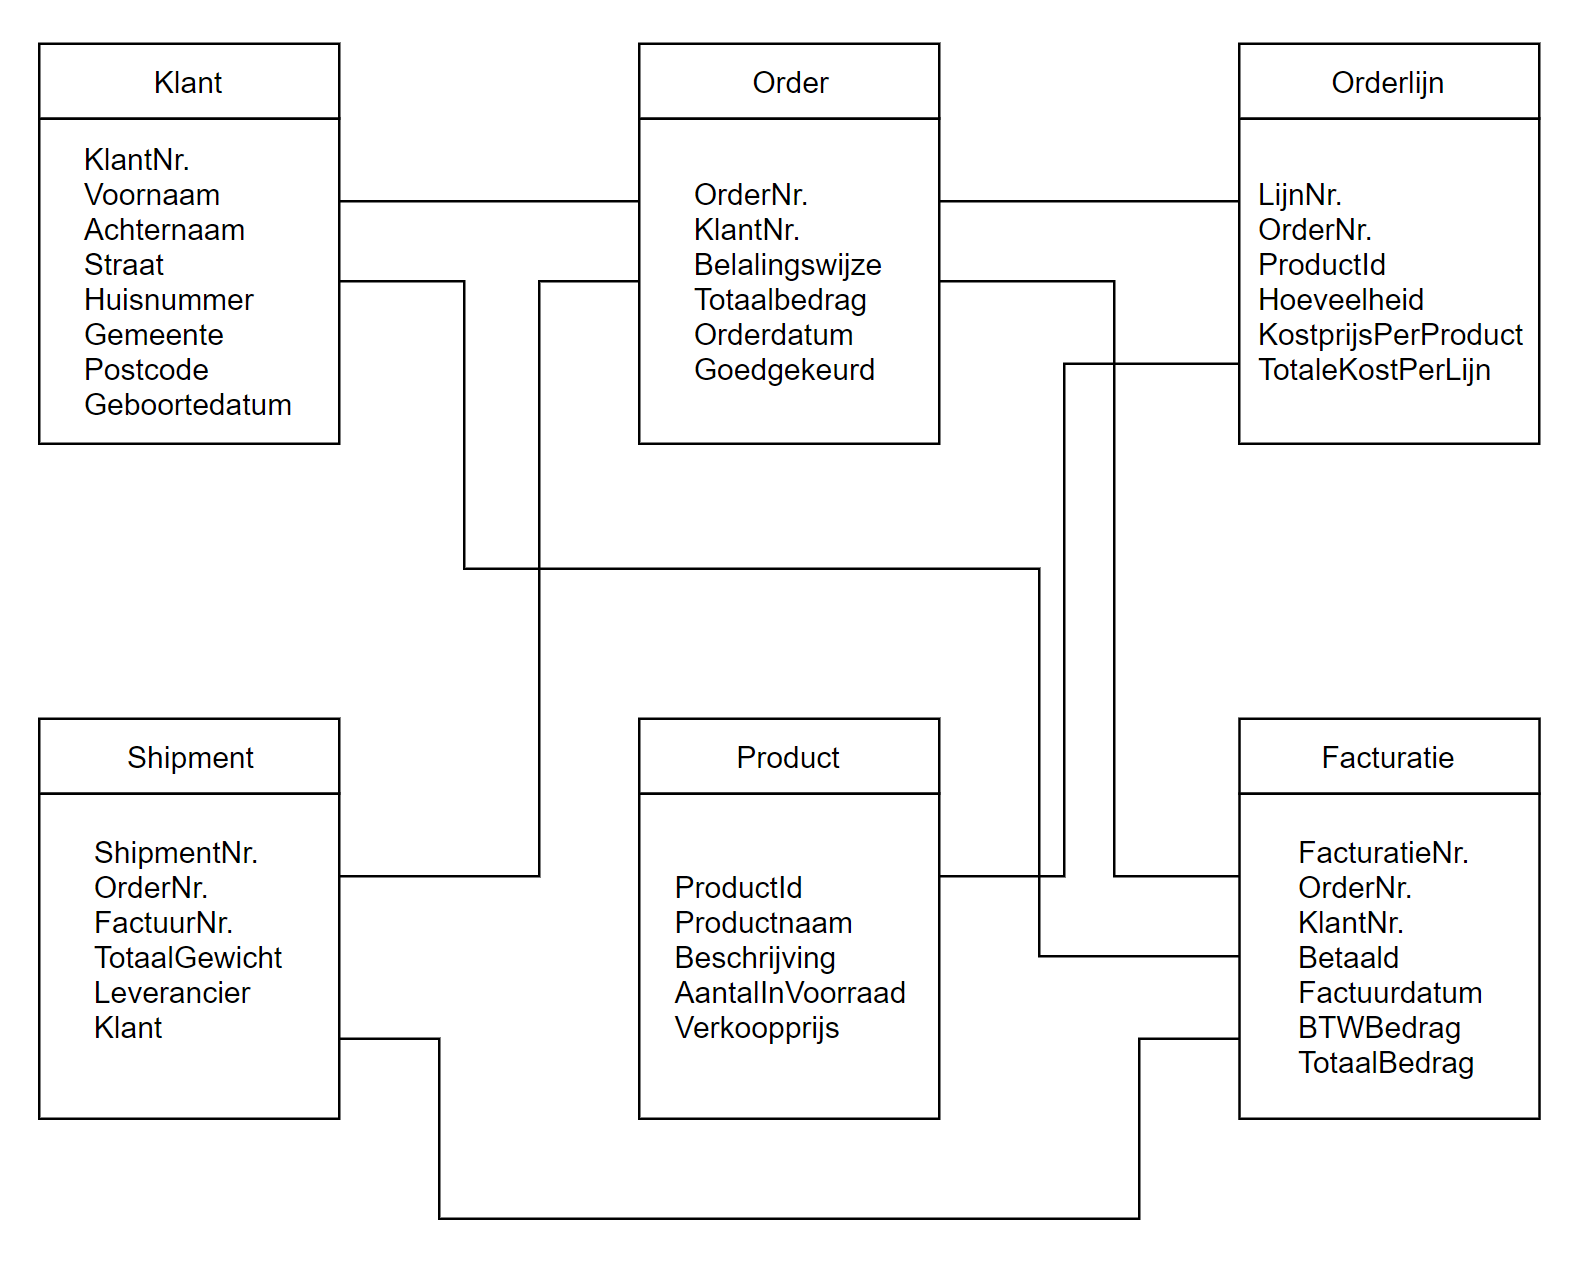
\includegraphics[width=15cm]{databank.png}
	\caption{De databank structuur.}
	\centering
\end{figure}

Aan de hand van het klantnummer is er geweten welk order tot een klant behoort. Credit management kan de eigenschap bij het order veranderen van 'goedgekeurd' naar 'niet goedgekeurd'. Van ieder order wordt een orderlijn bijgehouden waaraan een product of service is verbonden. Naast het product is ook een beschrijving en verkoopprijs te vinden. Het aantal in voorraad van ieder product is gekend omdat dit moet aangepast worden bij order fullfilment. De klantengegevens moeten gekend zijn om naar het juiste adres te factureren.

Elke databank heeft een queue. Wanneer microservice B iets nodig heeft van microservice A, kan die vraag naar de queue gepost worden.

De databank van microservice 'klant gegevens ophalen' zal alle data van de klanten bevatten.

De databank van microservice 'order plaatsen, ophalen en verwijderen' zal alle data van de orders bevatten.

De databank van microservice 'producten ophalen en aantal in de voorraad veranderen' zal alle data van de producten bevatten.

De databank van microservice 'facturatie maken en ophalen' alle data van de facturatie bevatten.

De databank van microservice 'Shipment documentatie opstellen' bevat de data van de orders om aan de hand van die data, de documenten op te stellen en dan toe te voegen aan de data met alle shipment documenten.

De databank van microservice 'Aanmaning opmaken en verwijderen' bevat alle data van de aanmaningen. 

De microservices 'bericht op queue plaatsen' en 'bericht van de queue halen', hebben geen datastore. Het zijn twee microservices die geen data moeten gaan ophalen of wegschrijven. Ze staan in voor het ophalen en plaatsen van berichten. 

\section{Communicatie tussen de microservices}
De communicatie gebeurt aan de hand van messaging. Aangezien order-to-cash een proces is waarin alleen voorwaarts kan worden gegaan, is er geen nood aan een message broker. Maar er wordt wel gewerkt met een queue. Daardoor raakt de microservices niet overbelast. Iedere microservice kan dan immers op zijn eigen tempo werken.
 
In het onderstaand voorbeeld heeft klant 66 geplaatst een order met vier verschillende producten. Het ordernummer is 23. De volledige bestelling komt binnen in het systeem en wordt op de queue van ordermanagement geplaatst. Het order wordt van de queue gehaald aan de hand van consumption en acknowledgement. Consumption betekent het bericht lezen. Acknowledgement is het bericht verwijderen. Ordermanagement verwerkt het binnengekomen order. Dan wordt het klantnummer en ordernummer op de queue van creditmanagement geplaatst. Creditmanagement haalt het bericht van de queue en kijkt naar het betaalgedrag van de klant. Staat de klant gekend voor wanbetalen, dan wordt er geen goedkeuring gegeven om het order te plaatsen. Bij een corect betaalgedrag, krijgt het order goedkeuring om geplaatst te worden. Dan wordt het ordernummer doorgestuurd naar het volgende deel van het proces. 
Dus volgende queue's zouden moeten bestaan:
\begin{itemize}
	\item QorderMan is een queue voor order management.
	\item QcreditMan is een queue voor credit management.
	\item QorderFul is een queue voor order fulfilment.
	\item QorderShip is een queue voor order shipment.
	\item Qfact is een queue voor de facturatie.
	\item QaccountsRec is een queue voor accounts receivable. 
\end{itemize}

Niet alle data wordt volledig naar de queue van de volgende stap gestuurd. Enkel belangrijke data zoals het klantennummer wordt verstuurd naar creditmanagement. Daar worden dan aan de hand van het klantnummer de bestelgegevens opgehaald en wordt nagegaan of die klant wel een order mag plaatsen. Het ordernummer wordt meegestuurd om zeker te zijn dat het correcte order goed- of afgekeurd wordt. Zo blijft de overhead op de queue minimaal. Om specifieke gegevens op te halen, moet de databank aangesproken worden. De gehele structuur van de databank wordt hieronder beschreven.

\subsection{De communicatie tussen de onderdelen van het OTC proces}

\begin{figure}[h!]
	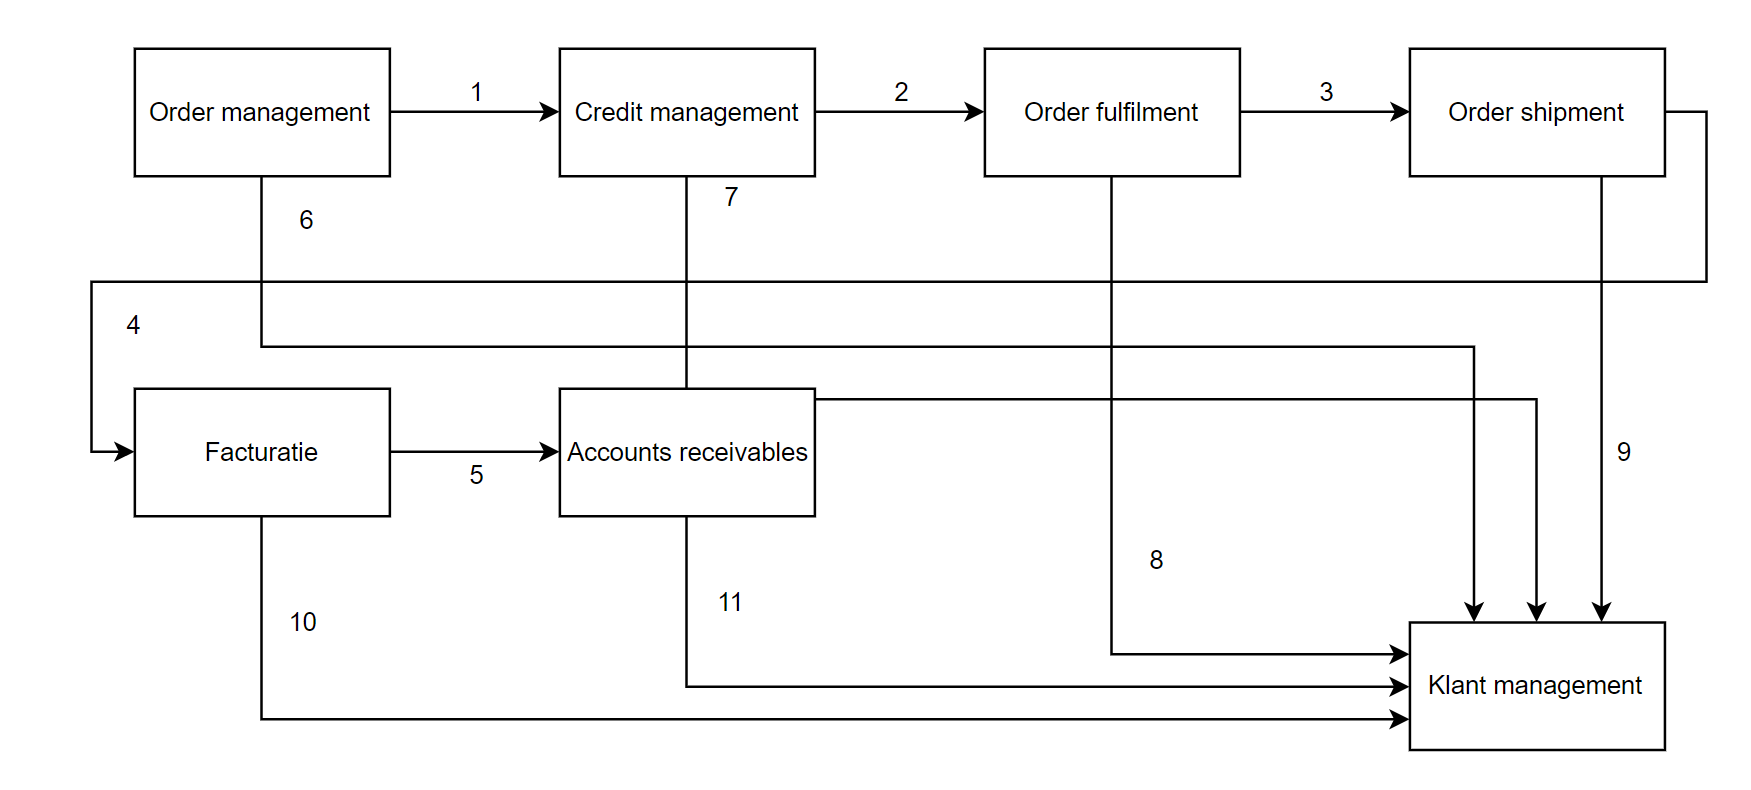
\includegraphics[width=15cm]{schema_communicatie.png}
	\caption{De communicatie tussen de verschillende onderdelen van het order-to-cash proces.}
	\centering
\end{figure}
Zoals eerder vermeld, is elk onderdeel van het OTC proces een microservice, die spreekt dan op zijn beurt kleinere microservices aan.
Op figuur 3.2 is het communicatiepatroon zichtbaar.
Vooraleer het proces van start kan gaan, moet een klant een order plaatsen. Een order bevat een aantal producten. Eens de klant een order geplaatst heeft, wordt er een ordernummer gemaakt. Belangrijk hierbij is dat er telkens een ordernummer verzonden wordt aan een onderdeel.
In het volgende hoofdstuk zullen de verschillende onderdelen uitgebreid beschrijven worden.
De nummers van de opsomming komen overeen met die op afbeelding 3.2.
\begin{enumerate}
	\item De communicatie tussen ordermanagement en creditmanagement. Er is een order geplaatst door klant 66. Ordermanagement zorgt ervoor dat het order in de databank geraakt. Daarna wordt het klantnummmer en het ordernummer op de queue van creditmanagement geplaatst. 
	\item De communicatie tussen creditmanagement en order fullfilment. Creditmanagement heeft het ordernummer en klantnummer van ordermanagement gekregen. Het bericht wordt van de queue gehaald. Creditmanagement gaat dan aan de hand van de klantgegevens beslissen of de klant het order mag plaatsen of niet. Is het order goedgekeurd, dan wordt het ordernummer op de queue van order fullfilment gezet.
	\item De communicatie tussen order fullfilment en order shipment. Order fullfilment heeft het ordernummer doorgekregen van credit management. Deze geeft het ordernummer op zijn beurt door aan order shipment eens zijn taak gedaan is. 
	\item De communicatie tussen order shipment en facturatie. Het ordernummer wordt op de queue van order shipment geplaatst. Eens alle documenten opgemaakt zijn bij order shipment, wordt het ordernummer doorgestuurd naar de facturatie.
	\item De communicatie tussen facturatie en accounts receivables. De facturatie kreeg een bericht van order shipment om de factuur op te maken voor het order met des betreffend ordernummer. Is de taak van facturatie afgerond, dan wordt het factuurnummer doorgestuurd naar accounts receivables. Op die manier aan de betaling verder opgevolgd worden.
	\item Ordermanagement plaatst het ordernummer op de queue van klant management. Klant management stuurt een bevestiging naar de klant en laat weten dat er eerst een controle komt op het betaalbedrag van de klant.
	\item Creditmanagement plaatst het ordernummer en de status van goedgekeurd of afgekeurd op de queue. Deze status wordt in een bericht naar de klant verzonden. 
	\item Order fullfilment plaatst een bericht op de queue om te laten weten dat de goederen uit het magazijn werden opgehaald en klaar staan voor verzending.
	\item Order shipment plaatst een bericht op de queue wanneer de goederen klaar zijn voor vertrek. Klant management zorgt er dan voor dat het bericht tot bij de klant geraakt.
	\item Facturatie plaatst een bericht op de queue van klant management om ervoor te zorgen dat de factuur tot bij de klant geraakt.
	\item Accounts receivables plaatst een bericht op de queue van klant management als er aanmaningen moeten worden gestuurd.
\end{enumerate}

\subsection{De architectuur}
In volgende tabel zijn letters en bijhorende microservices terug te vinden. Deze worden gebruikt bij het uitleggen van de architectuur.
\begin{table}[]
	\resizebox{\textwidth}{!}{%
		\begin{tabular}{|l|p{15cm}|}
			\hline 
			A & Klantgegevens ophalen \\ \hline
			B & Orders plaatsen, ophalen en verwijderen \\ \hline
			C & Producten ophalen en het aantal op voorraad aanpassen \\ \hline
			D & Shipment documenten opstellen \\ \hline
			E & Facturatie maken en ophalen \\ \hline
			F & Aanmaning opmaken en verwijderen \\ \hline
			G & Bericht plaatsen op de queue \\ \hline
			H & Bericht ophalen uit de queue \\ \hline
		\end{tabular}%
	}
	\caption{Legende die gebruikt wordt in de afbeeldingen.}
\end{table}

In tabel 3.1 is de legende terug te vinden die gebruikt wordt bij het uitleggen van elk onderdeel.
In figuur 3.3 is te zien hoe het volledige proces communiceert met de verschillende microservices. Elk onderdeel van het proces is een microservice op zich.
\begin{figure}[h!]
	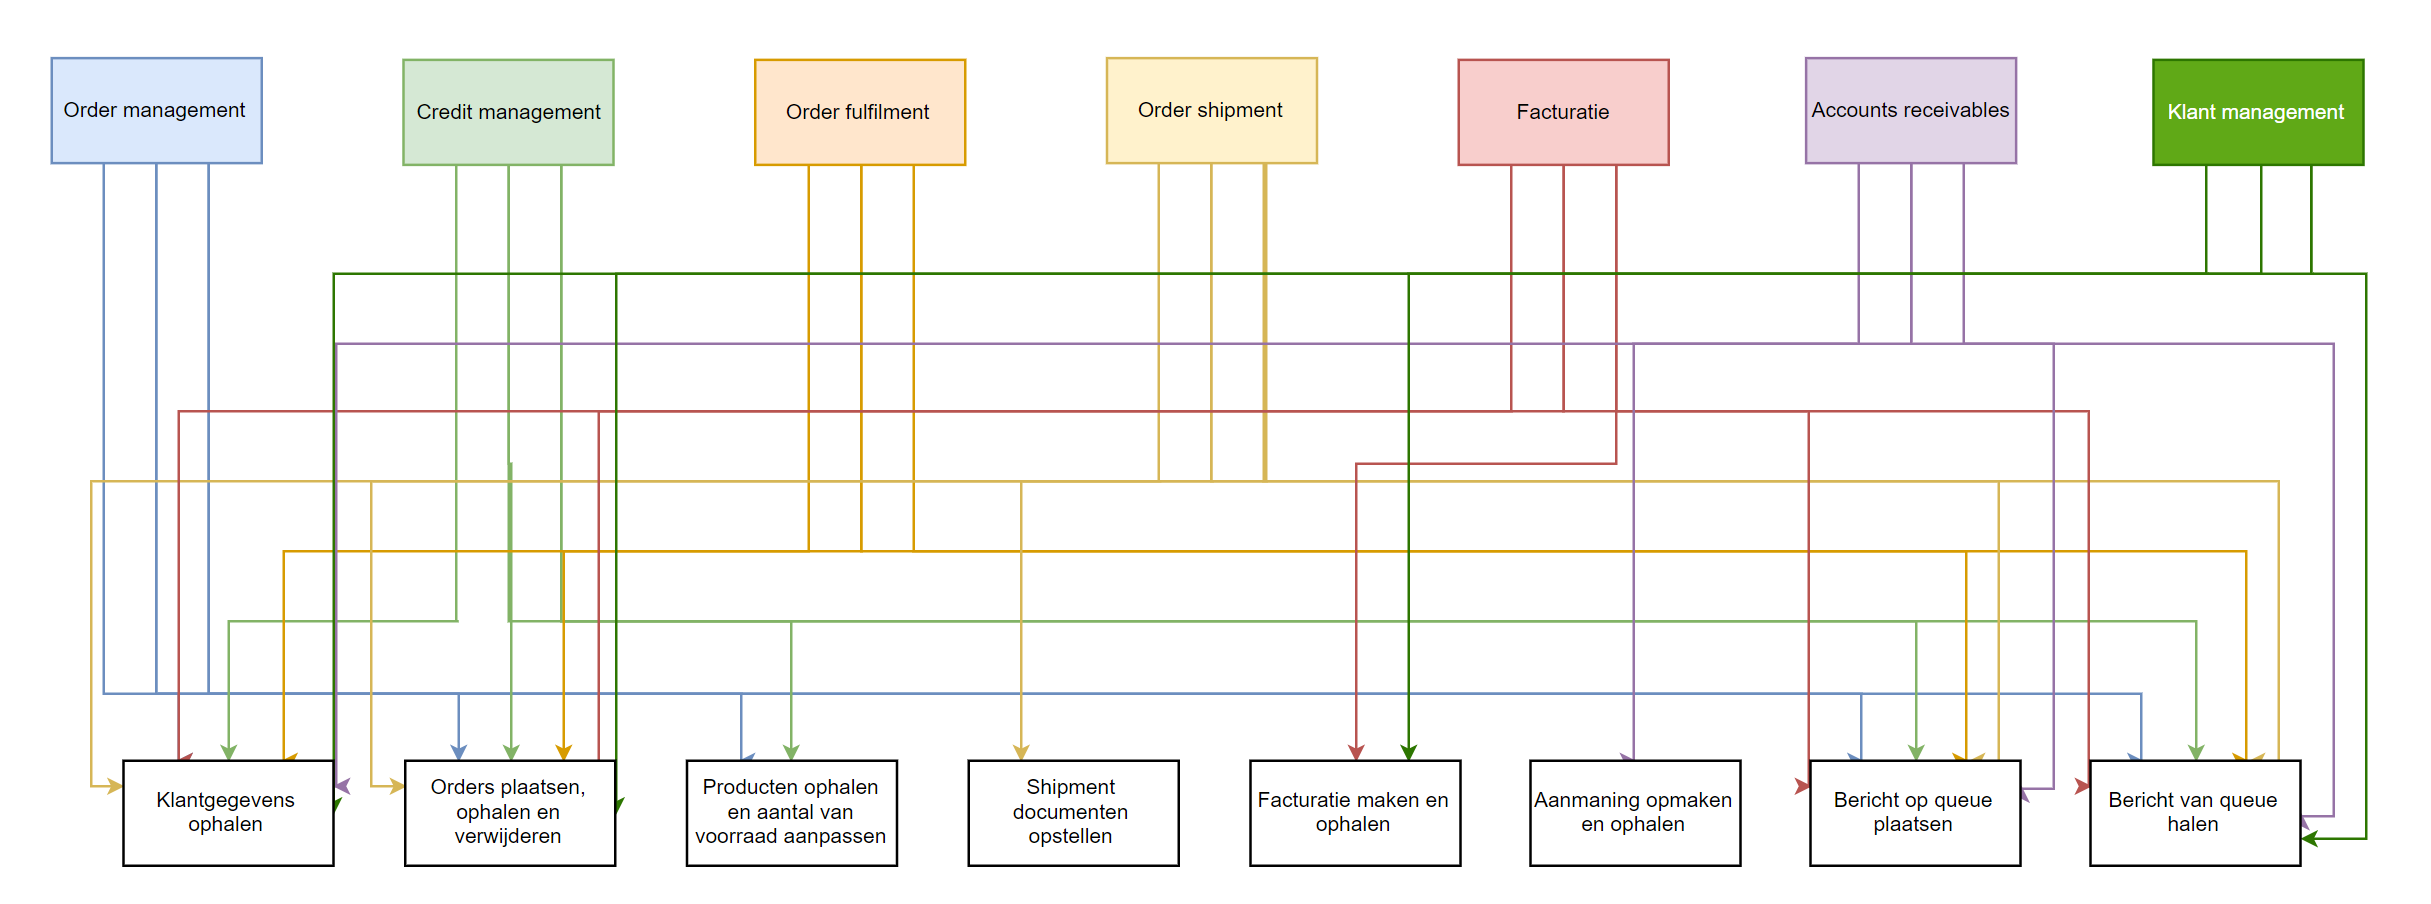
\includegraphics[width=15cm]{schema_microservices.png}
	\caption{Welk onderdeel welke microservices aanspreekt.}
	\centering
\end{figure}

\subsubsection{Order management}
\begin{figure}[h!]
	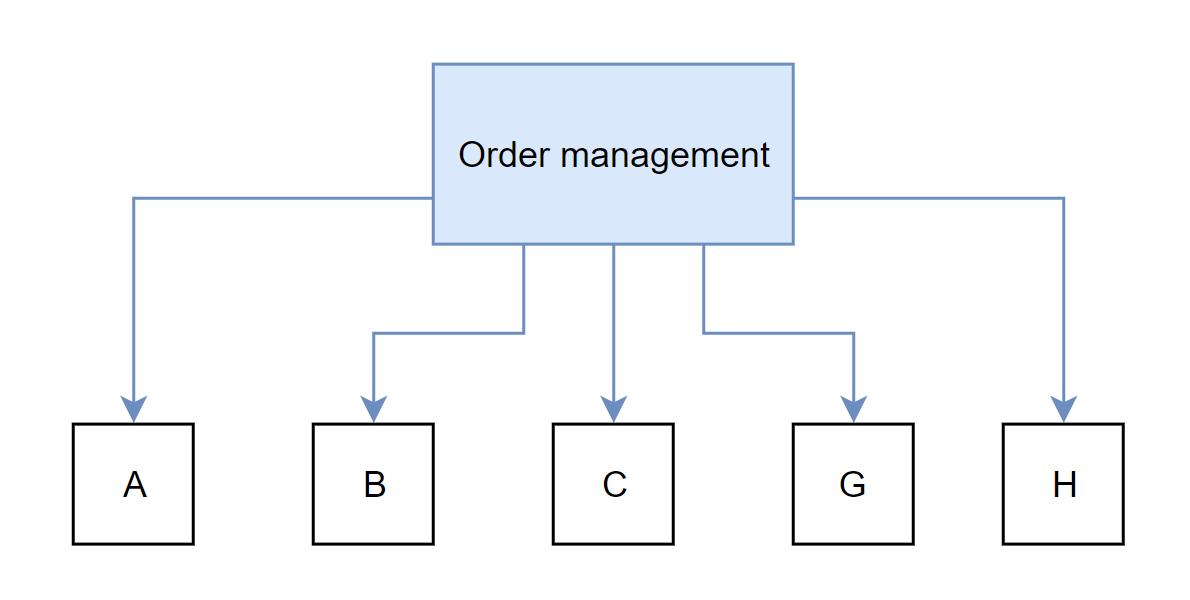
\includegraphics[width=5cm]{ordermanagement.png}
	\caption{Order management communiceert met volgende microservices.}
	\centering
\end{figure}
Order management communiceert met volgende microservices:
\begin{itemize}
	\item Klantengegevens ophalen.
	\item Orders plaatsen, ophalen en verwijderen.
	\item Producten ophalen en het aantal van de voorraad aanpassen.
	\item Bericht plaatsen op queue.
	\item Bericht van queue halen.
\end{itemize}
Een klant plaatst een order op het platform van het bedrijf. De gegevens van de klant worden opgehaald en gelinkt aan het nieuw gecreëerde order. Eens die twee taken zijn afgerond, wordt het bericht op de queue geplaatst van credit management.

\subsubsection{Credit management}
\begin{figure}[h!]
	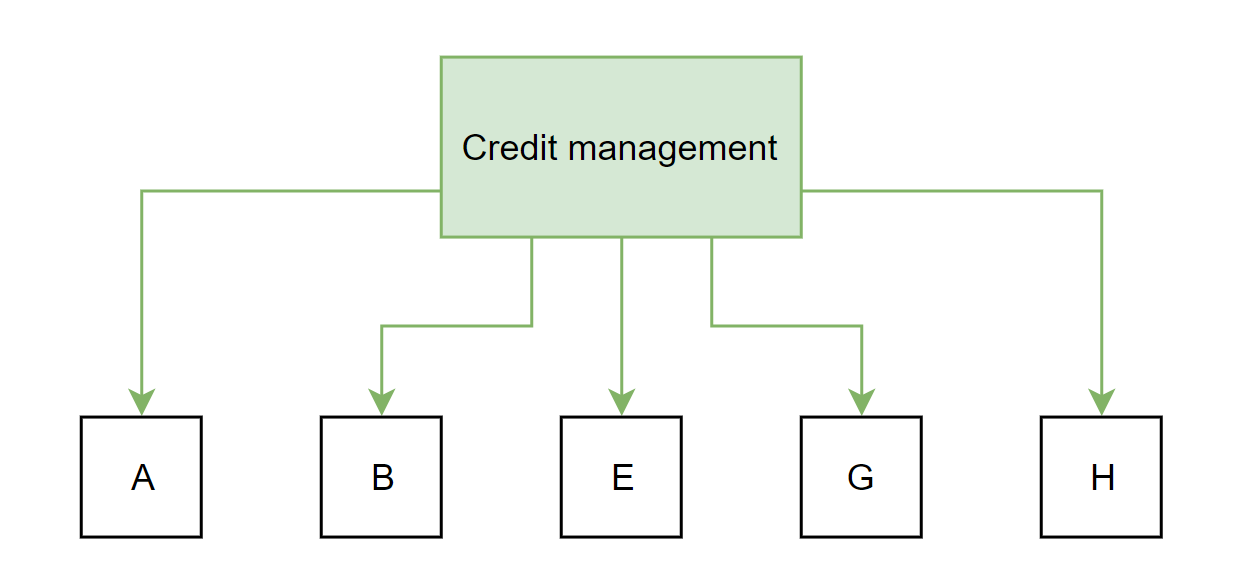
\includegraphics[width=5cm]{creditmanagement.png}
	\caption{Credit management communiceert met volgende microservices.}
	\centering
\end{figure}
Credit management communiceert met volgende microservices:
\begin{itemize}
	\item Klantengegevens ophalen.
	\item Orders ophalen, plaatsen en verwijderen.
	\item Facturatie maken en ophalen.
	\item Bericht plaatsen op queue.
	\item Bericht van queue halen.
\end{itemize}
Eerst wordt het bericht opgehaald dat order management op de queue plaatste. Daarna wordt er een klantennummer en ordernummer verzonden. Credit management kijkt of de klant een goed betaalgedrag heeft. Is de klant bekend als wanbetaler dan wordt het order afgekeurd. In andere gevallen krijgt het order een goedkeuring en wordt het ordernummer geplaatst op de queue van order fullfilment. Dan zit de taak van credit management erop.

\subsubsection{Order fullfilment}
\begin{figure}[h!]
	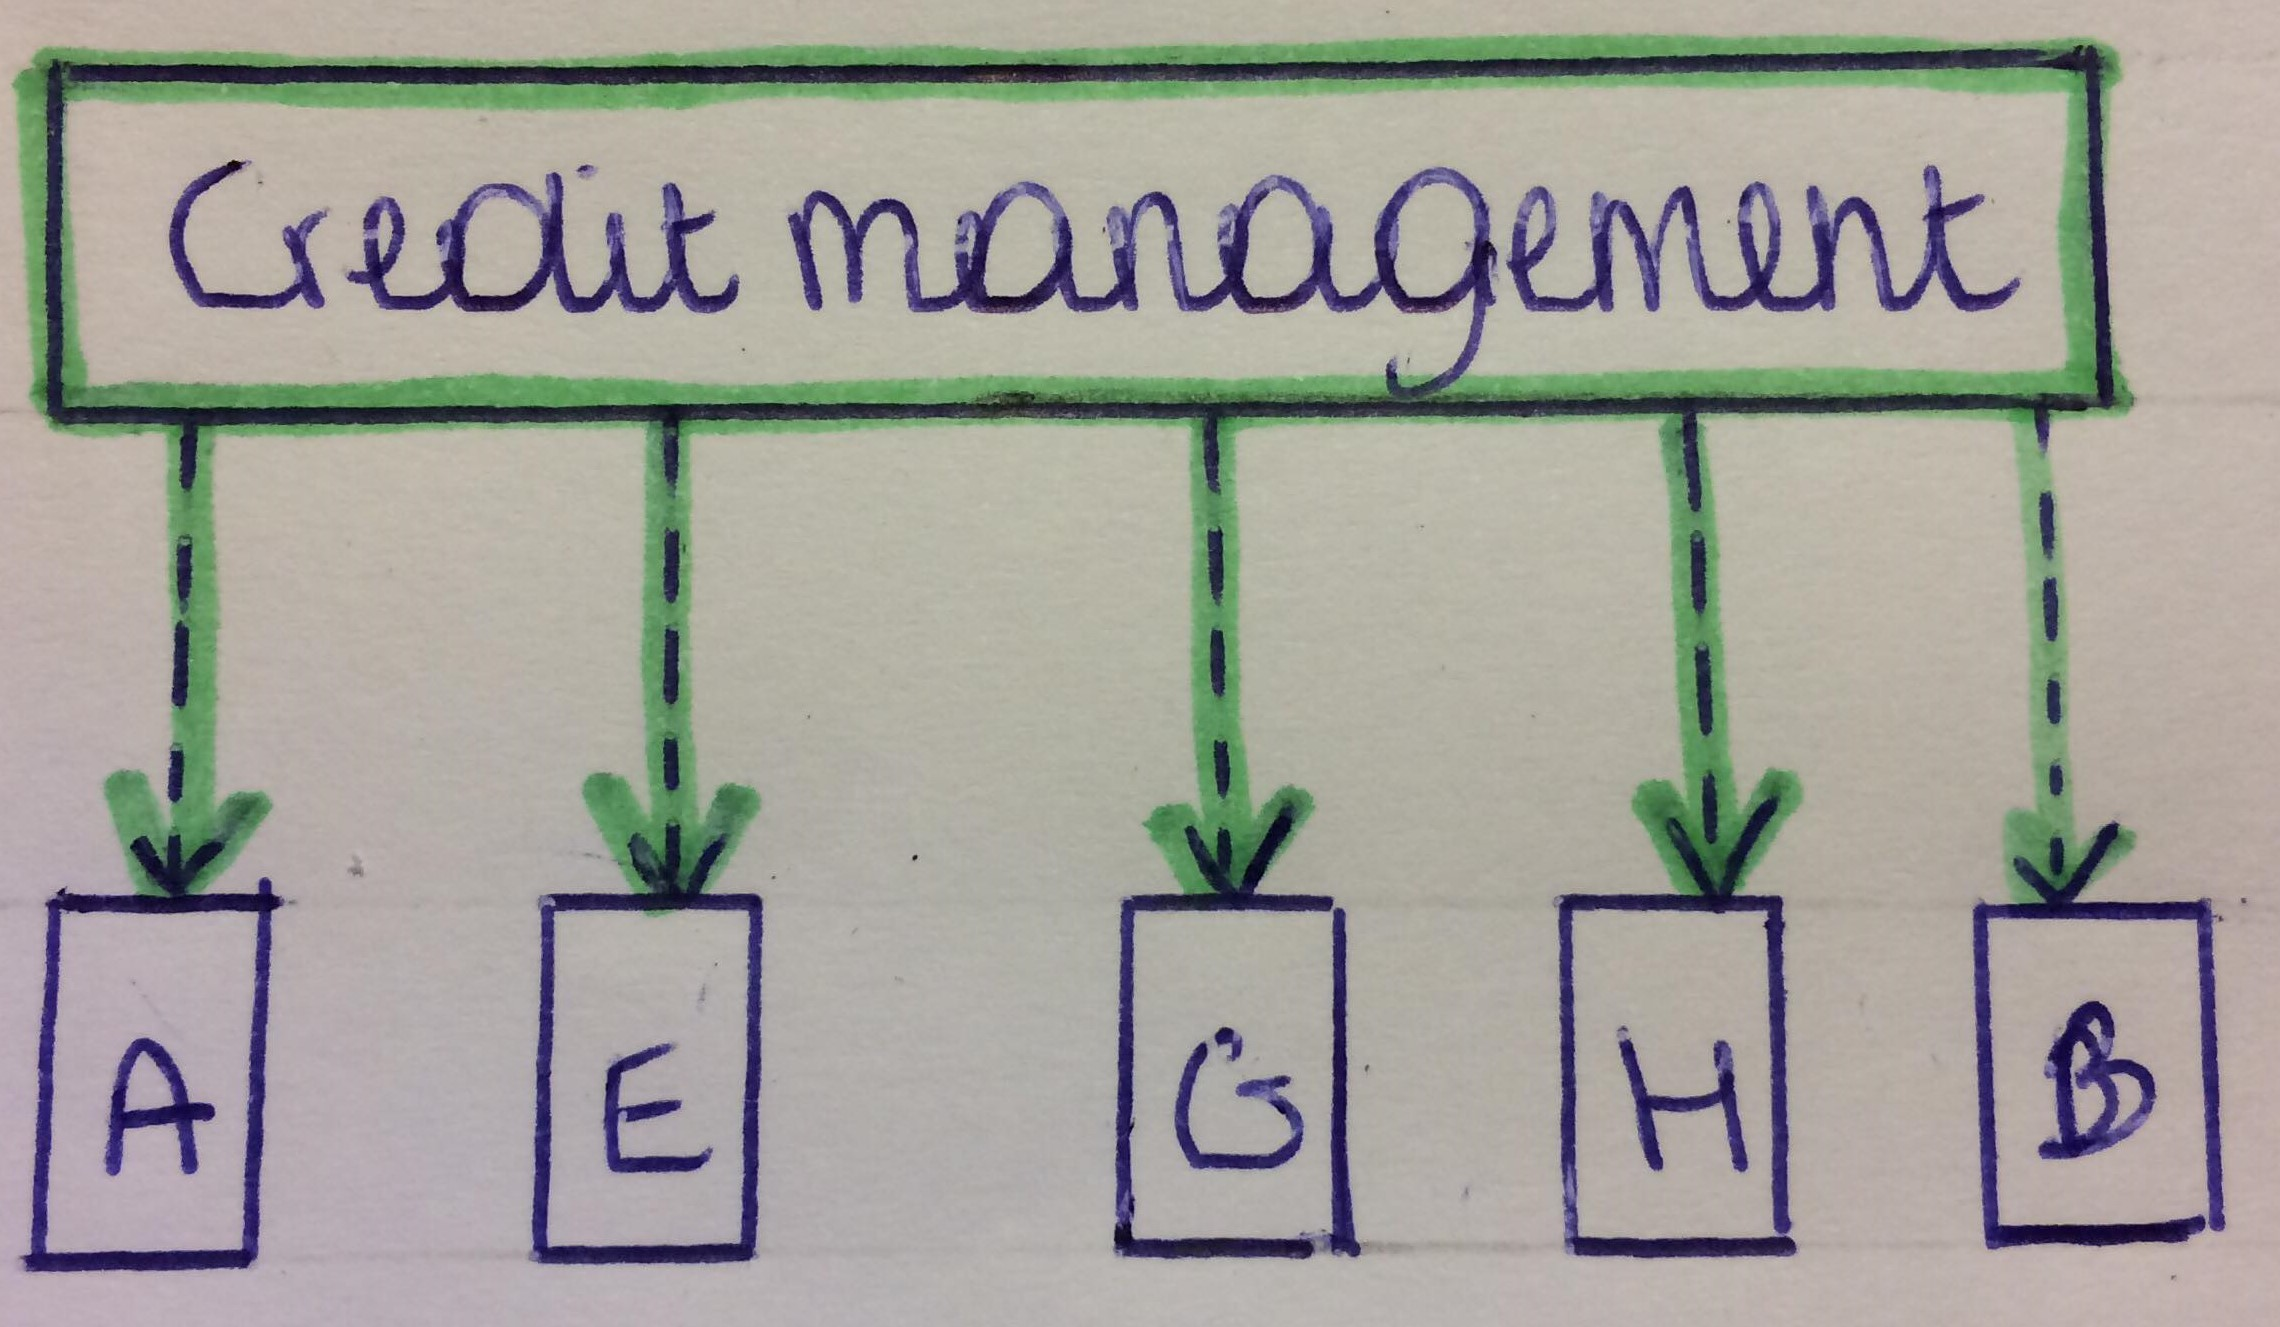
\includegraphics[width=5cm]{orderfullfilment.png}
	\caption{Order fullfilment communiceert met volgende microservices.}
	\centering
\end{figure}
Order fullfilment communiceert met volgende microservices:
\begin{itemize}
	\item Orders ophalen, plaatsen en verwijderen.
	\item Producten ophalen en het aantal in de voorraad aanpassen.
	\item Bericht plaatsen op queue.
	\item Bericht van queue halen.
\end{itemize}
Bij order fullfilment staat een ordernummer op de queue. Dit wordt opgehaald en geef aan welke goederen er uit het magazijn moeten gehaald worden. Voor alle goederen moet het aantal in de voorraad aangepast worden. Eens het order compleet is, wordt het ordernummer op de queue van order shipment geplaatst.

\subsubsection{Order shipment}
\begin{figure}[h!]
	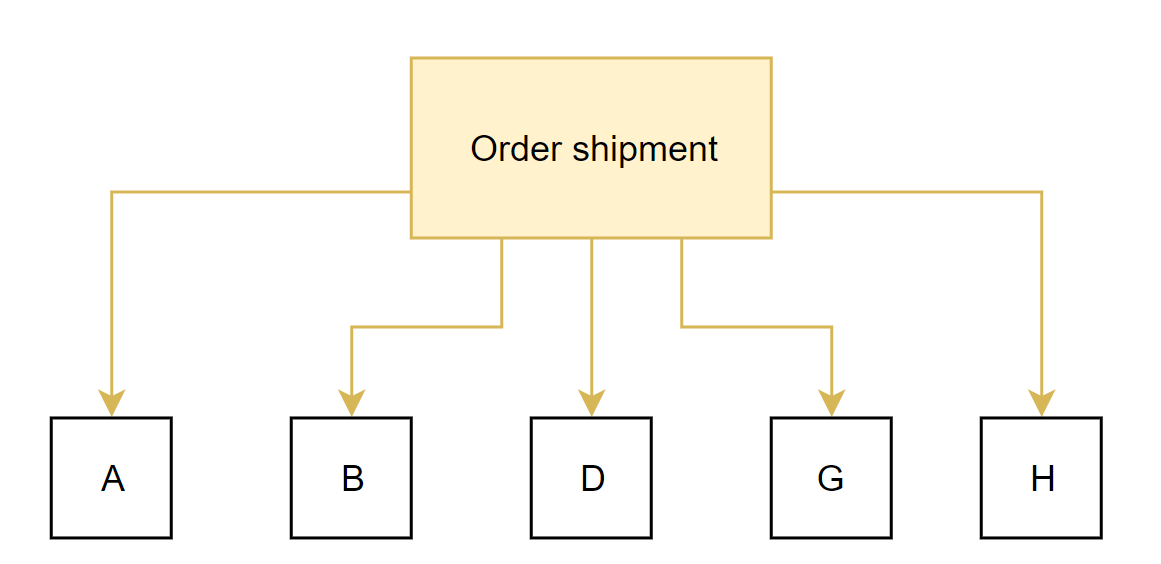
\includegraphics[width=5cm]{ordershipment.png}
	\caption{Order shipment communiceert met volgende microservices.}
	\centering
\end{figure}
Order shipment communiceert met volgende microservices:
\begin{itemize}
	\item Orders ophalen, plaatsen en verwijderen.
	\item Klantengegevens ophalen.
	\item Shipment document opstellen.
	\item Bericht plaatsen op queue.
	\item Bericht van queue halen.
\end{itemize}
Order shipment krijgt het ordernummer binnen via zijn queue. Het order wordt bekeken en de klantengegevens worden opgehaald aan de hand van het klantnummer dat gekoppeld werd aan het order. Eens het order shipment document is opgesteld en alle goederen klaar zijn voor vertrek, wordt het ordernummer geplaatst op de queue van facturatie.

\subsubsection{Facturatie}
\begin{figure}[h!]
	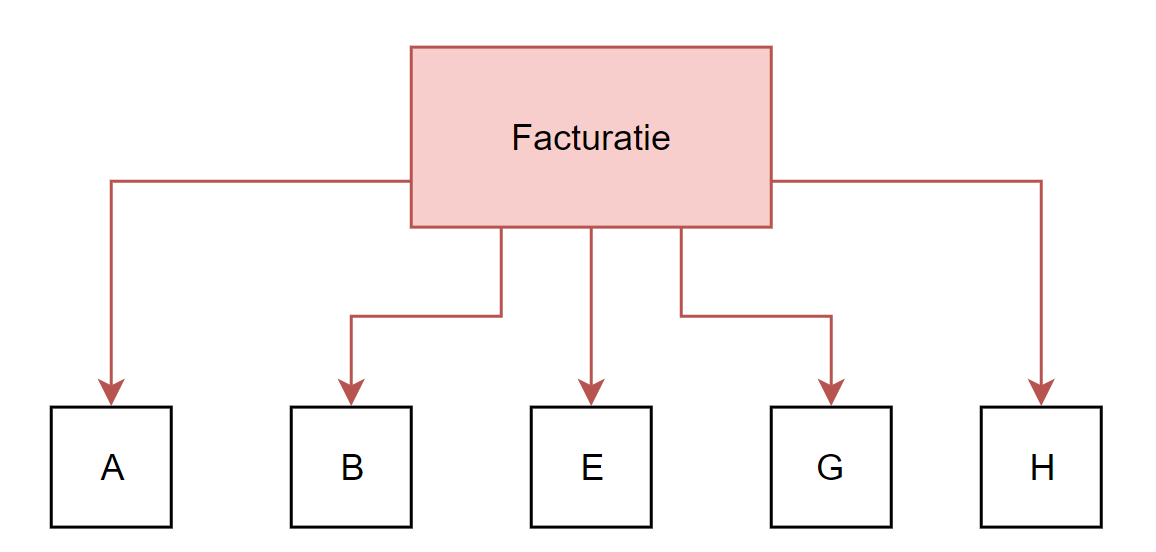
\includegraphics[width=5cm]{facturatie.png}
	\caption{Facturatie communiceert met volgende microservices.}
	\centering
\end{figure}
Facturatie communiceert met volgende microservices:
\begin{itemize}
	\item Klantengegevens ophalen.
	\item Orders ophalen, plaatsen en verwijderen.
	\item Facturen maken en ophalen.
	\item Bericht plaatsen op queue.
	\item Bericht van queue halen.
\end{itemize}
Eens het ordernummer opgehaald is van de queue, wordt alle nodig info opgehaald om de factuur op te maken. De nodige gegevens zijn klantengegevens en het order. Eens de factuur opgemaakt is, wordt het factuur nummer geplaatst op de queue van account receivables.

\subsubsection{Accounts receivables}
\begin{figure}[h!]
	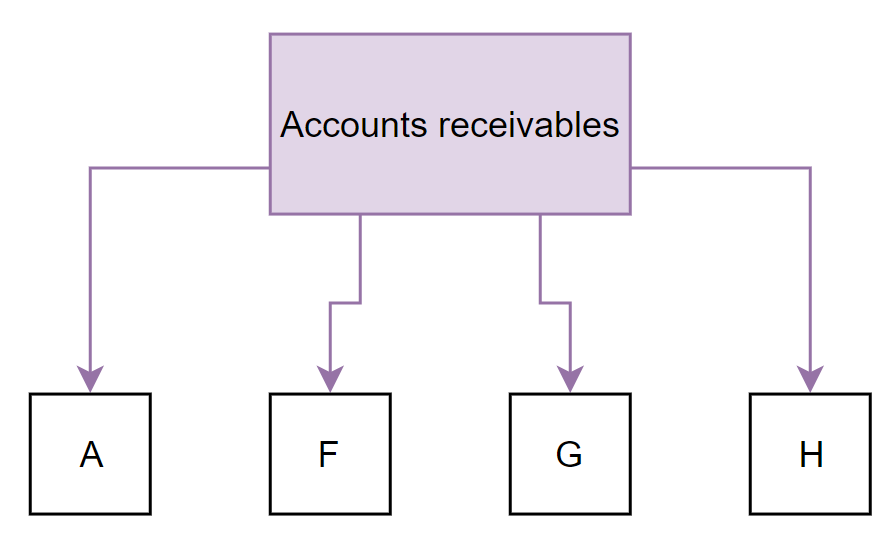
\includegraphics[width=5cm]{accountreceivables.png}
	\caption{Accounts receivables communiceert met volgende microservices.}
	\centering
\end{figure}
Accounts receivable gaat na of de betaling wel goed wordt afgerond. Hiervoor worden volgende microservices aangesproken:
\begin{itemize}
	\item Klantengegevens ophalen.
	\item Facturen maken en ophalen.
	\item Bericht plaatsen op queue.
	\item Bericht van queue halen.
\end{itemize}

\subsubsection{Klant management}
\begin{figure}[h!]
	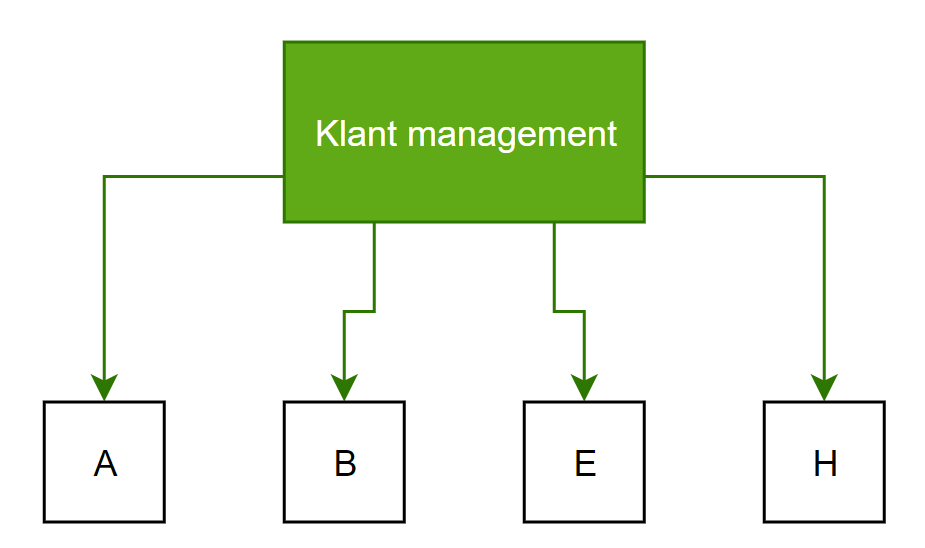
\includegraphics[width=5cm]{klantmanagement.png}
	\caption{Klant management communiceert met volgende microservices.}
	\centering
\end{figure}
Klant management staat in voor het contact met de klant. Dit onderdeel gebruikt volgende microservices:
\begin{itemize}
	\item Klanentgegevens ophalen.
	\item Orders ophalen, plaatsen en verwijderen.
	\item Facturen maken en ophalen.
	\item Bericht van queue halen.
\end{itemize}
Als een van de vorige onderdelen een bericht plaatst op deze queue, zal het bericht verwerkt worden. Daarna wordt de klant verwittigd met de inhoud van het bericht. Als de klant bijvoorbeeld geen order mag bestellen omdat credit management nog onbetaalde facturen gevonden heeft, wordt de klant hiervan op de hoogte gebracht via klant management.


\section{De complete architectuur opbouwen}
Op figuur 3.11 is te zien hoe het proces in elkaar. Door de microservicearchitectuur toe te passen op het order-to-cash proces verandert er niks aan de volgorde van het proces. De manier waarop gegevens worden opgehaald, verandert wel. 


\subsection{De volgende stappen: Het toevoegen van API, logging en authenticatie en authorisatie}
\subsubsection{Logging}
Logging kan toegepast worden door nog een extra microservice te ontwikkelen. Hier kunnen de andere microservices dan hun logs naar posten. Dit wordt gebruikt om fouten in de architectuur te ontdekken. Hier zal echter niet verder op worden ingegaan. 

\subsubsection{API gateway}
Een API gateway wordt toegevoegd om ervoor te zorgen dat de architctuur niet openbaar is voor iedereen. Op die manier is er één aanspreekpunt en die regelt de rest van de communicatie.
De API communiceert in dit geval enkel met order management. Het geeft alle nodige informatie door en order management schrijft deze weg naar de databank.
\begin{figure}[h!]
	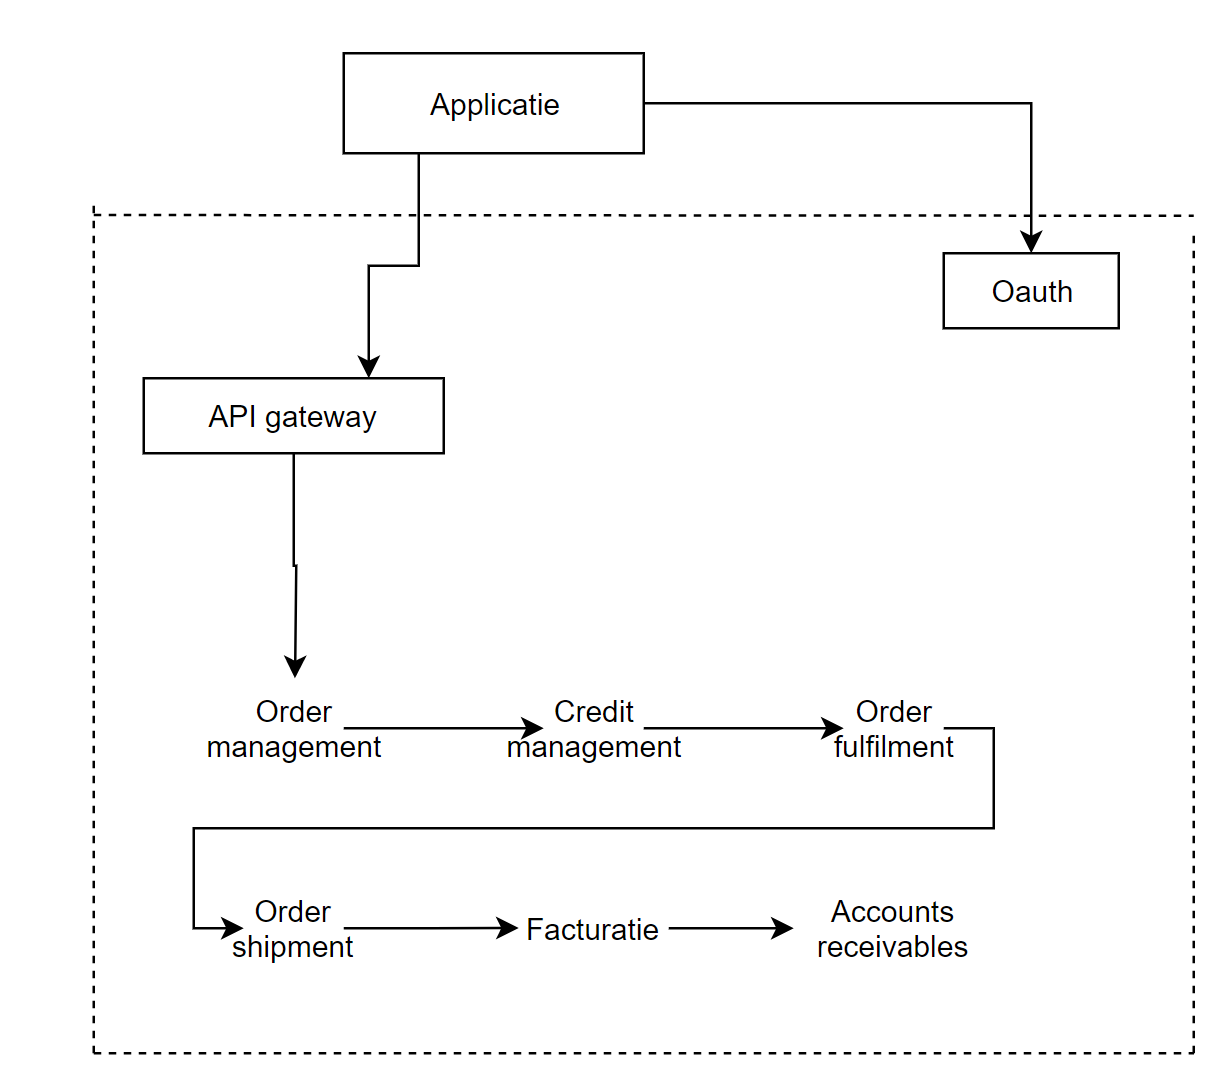
\includegraphics[width=10cm]{apiSchema.png}
	\caption{Vereenvoudigd schema.}
	\centering
\end{figure}

\subsubsection{Authenticatie en autorisatie}
Onder het hoofdstuk 'Stand Van Zaken', is er meer info te vinden over authenticatie. Uit die vergelijking, is API gekozen als authenticatie, specifiek voor OAuth omdat dit de meest bekende en gebruikte versie is.

De gebruiker moet gekend zijn om een order te kunnen plaatsen. Er is een aparte micrservice voor authenticatie. Hier wordt niet dieper op in gegaan omdat dit buiten de onderzoeksvraag van deze bachelorproef valt.



